\documentclass[12pt]{article}

\usepackage[a4paper, margin=1in]{geometry}
\usepackage{graphicx}
\usepackage{amsmath}
\usepackage{booktabs}
\usepackage{float}
\usepackage{hyperref}

\title{\textbf{Credit Card Fraud Detection:\\
Exploratory Data Analysis and Behavioral Profiling}}

\author{Nomusa Shongwe}
\date{}

\begin{document}

\maketitle

\begin{abstract}
Credit card fraud remains a significant challenge in modern financial systems. This study performs an in-depth exploratory data analysis (EDA) to identify behavioral patterns associated with fraudulent transactions. Results indicate that fraud is driven primarily by transaction context, including time, amount, and category, rather than demographic attributes. Fraudulent transactions are more frequent during late-night hours, involve higher monetary values, and are concentrated in online retail categories. Correlation analysis reveals weak linear relationships, emphasizing the need for multi-feature modeling approaches.
\end{abstract}

\section{Introduction}

With the rapid growth of digital transactions, fraud detection has become increasingly important. Traditional rule-based systems are insufficient due to evolving fraud strategies. Data-driven approaches, particularly machine learning, require a strong understanding of underlying data patterns.

This study applies exploratory data analysis to uncover fraud characteristics and inform predictive modeling.

\section{Methodology}

The analysis includes:
\begin{itemize}
    \item Data preprocessing and feature engineering
    \item Temporal analysis (hour, day, night)
    \item Demographic analysis (age)
    \item Category-based fraud analysis
    \item Correlation analysis
\end{itemize}

\section{Results and Discussion}

\subsection{Day vs Late-Night Fraud}

\begin{figure}[H]
\centering
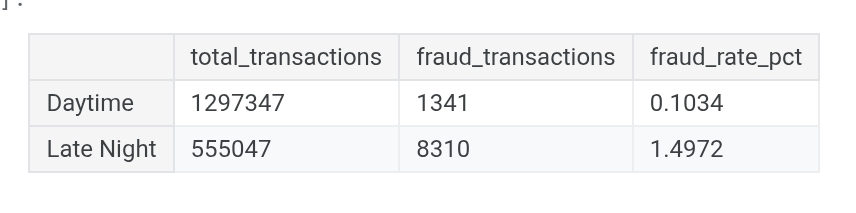
\includegraphics[width=0.8\textwidth]{figures/day_vs_night.png}
\caption{Daytime vs Late-Night Fraud Comparison}
\end{figure}

Fraud is significantly higher during late-night hours, with a fraud rate exceeding daytime activity by more than tenfold. This suggests exploitation of low-monitoring periods.

\subsection{Fraud Rate by Day of Week}

\begin{figure}[H]
\centering
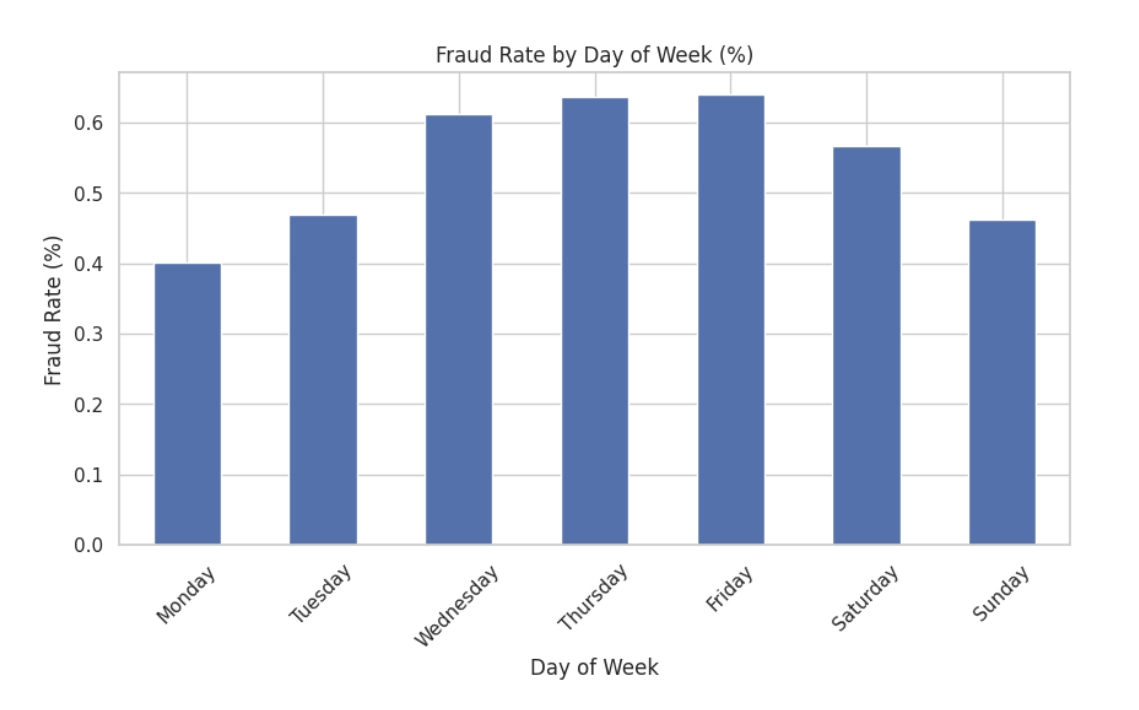
\includegraphics[width=0.8\textwidth]{figures/day_of_week.png}
\caption{Fraud Rate by Day of Week}
\end{figure}

Fraud increases through the week and peaks around Thursday and Friday, indicating alignment with higher transaction volumes.

\subsection{Customer Age Distribution}

\begin{figure}[H]
\centering
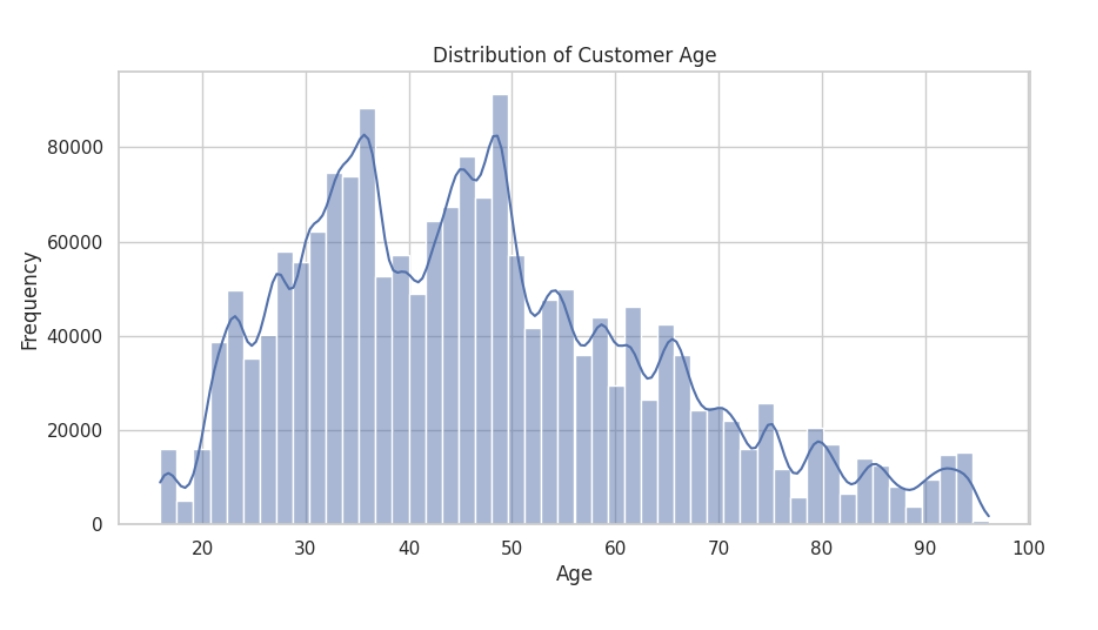
\includegraphics[width=0.8\textwidth]{figures/age_distribution.png}
\caption{Distribution of Customer Age}
\end{figure}

Most customers fall between ages 30 and 60.

\begin{figure}[H]
\centering
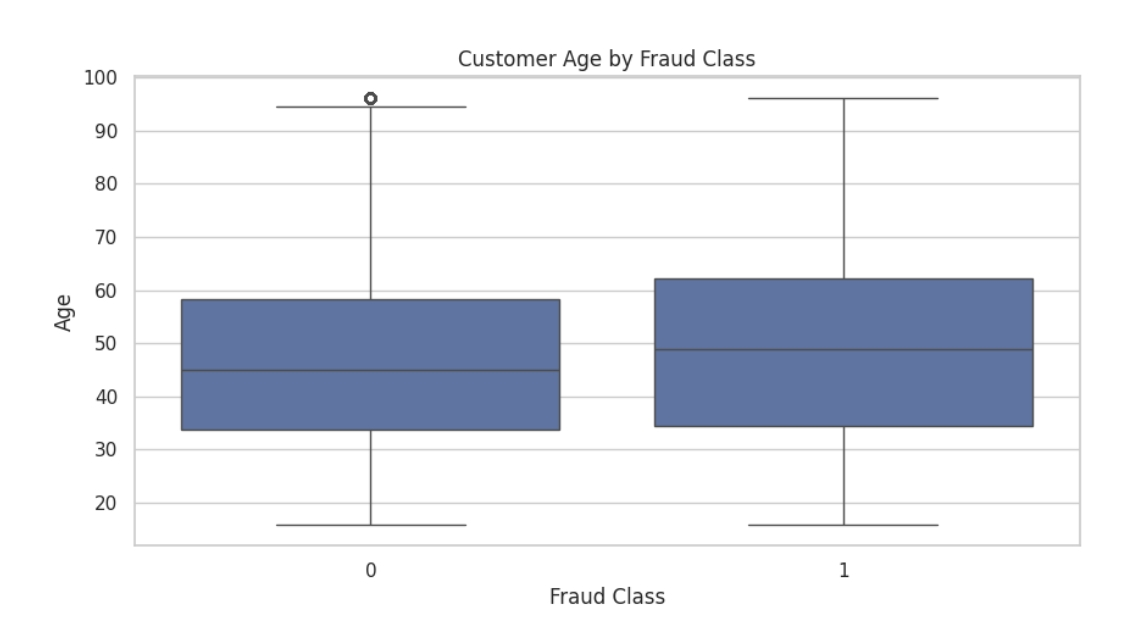
\includegraphics[width=0.8\textwidth]{figures/age_boxplot.png}
\caption{Customer Age by Fraud Class}
\end{figure}

There is significant overlap between fraud and non-fraud age distributions, indicating weak predictive power.

\subsection{Fraud Rate by Age Band}

\begin{figure}[H]
\centering
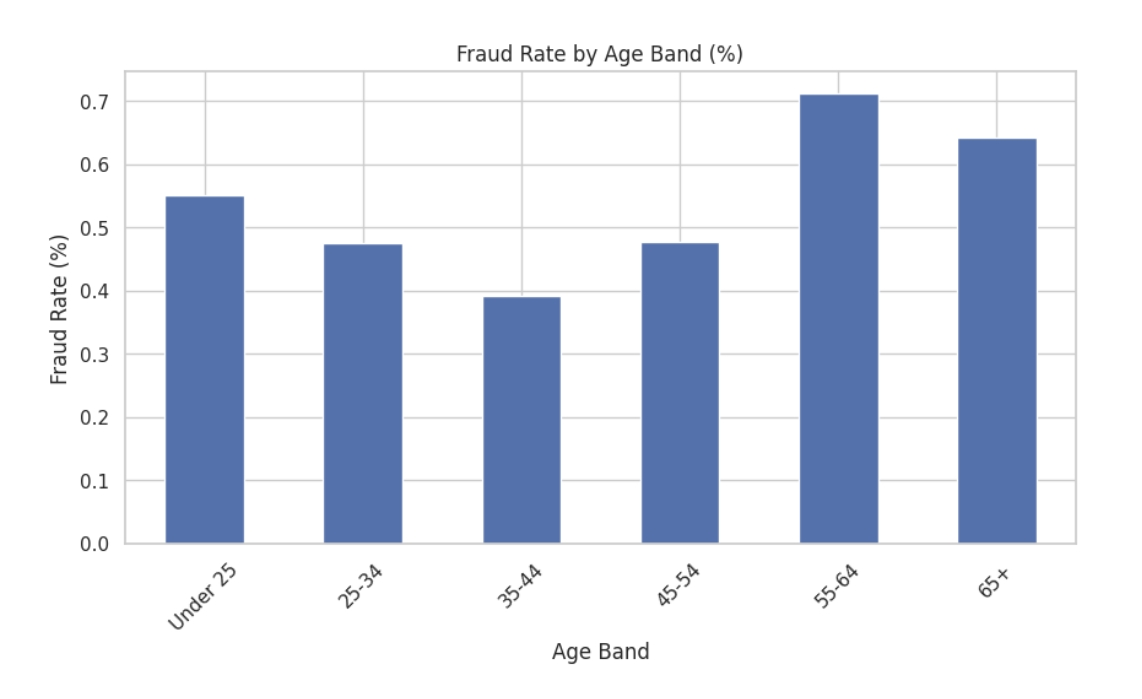
\includegraphics[width=0.8\textwidth]{figures/age_band.png}
\caption{Fraud Rate by Age Band}
\end{figure}

Older age groups show slightly higher fraud rates, but differences remain small.

\subsection{Fraud Transaction Amount Distribution}

\begin{figure}[H]
\centering
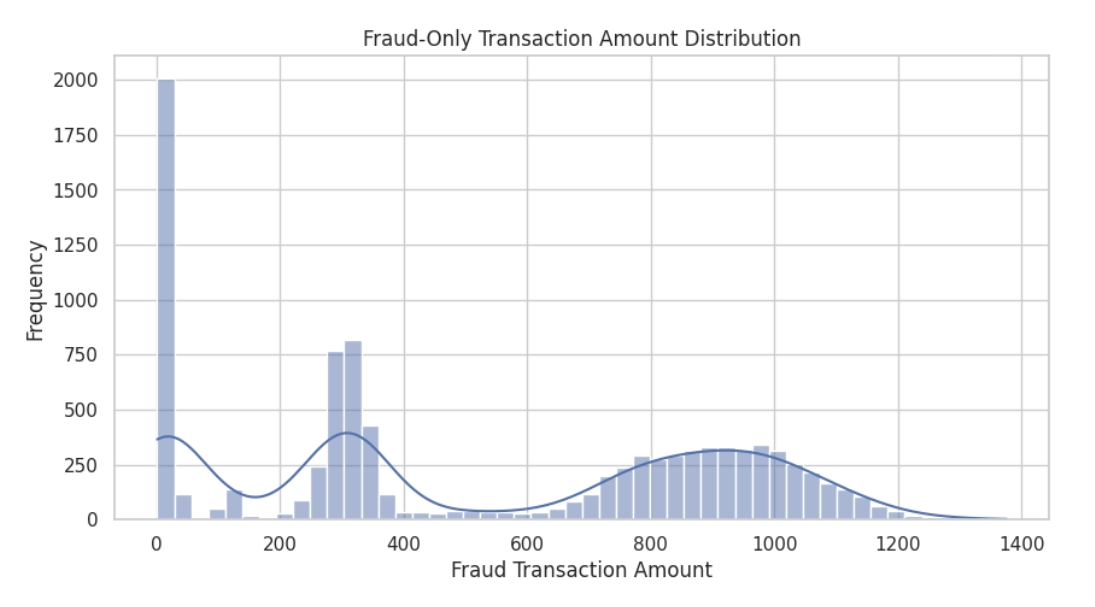
\includegraphics[width=0.8\textwidth]{figures/fraud_amount.png}
\caption{Fraud Transaction Amount Distribution}
\end{figure}

Fraudulent transactions are generally higher in value, supporting the hypothesis that fraudsters maximize returns.

\subsection{Fraud Categories}

\begin{figure}[H]
\centering
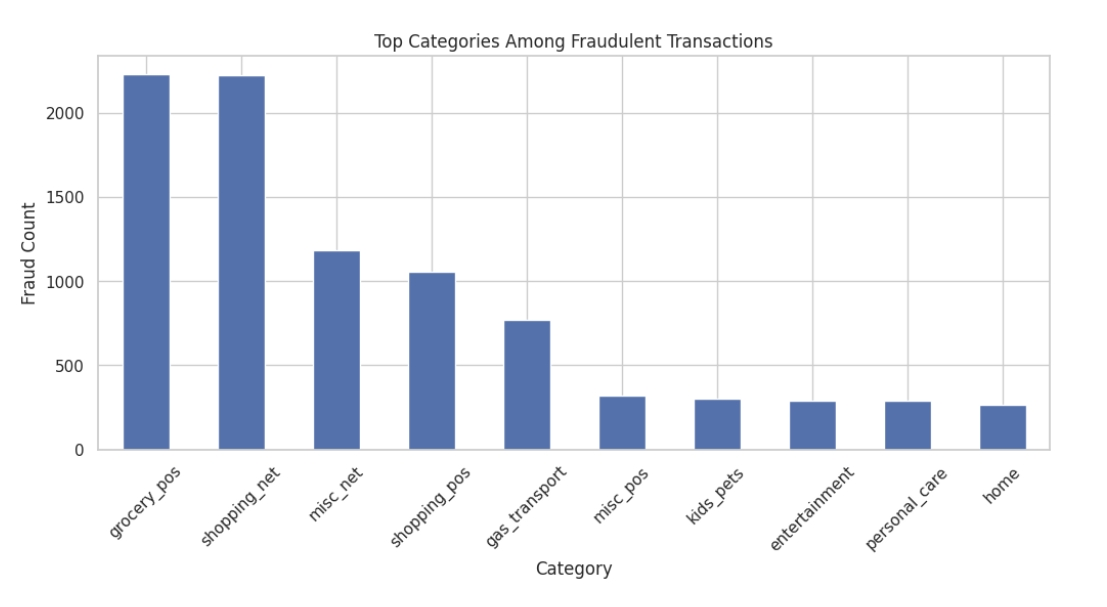
\includegraphics[width=0.8\textwidth]{figures/categories.png}
\caption{Top Fraud Categories}
\end{figure}

Fraud is concentrated in online and retail categories such as \texttt{shopping\_net} and \texttt{grocery\_pos}.

\subsection{Correlation Analysis}

\begin{figure}[H]
\centering
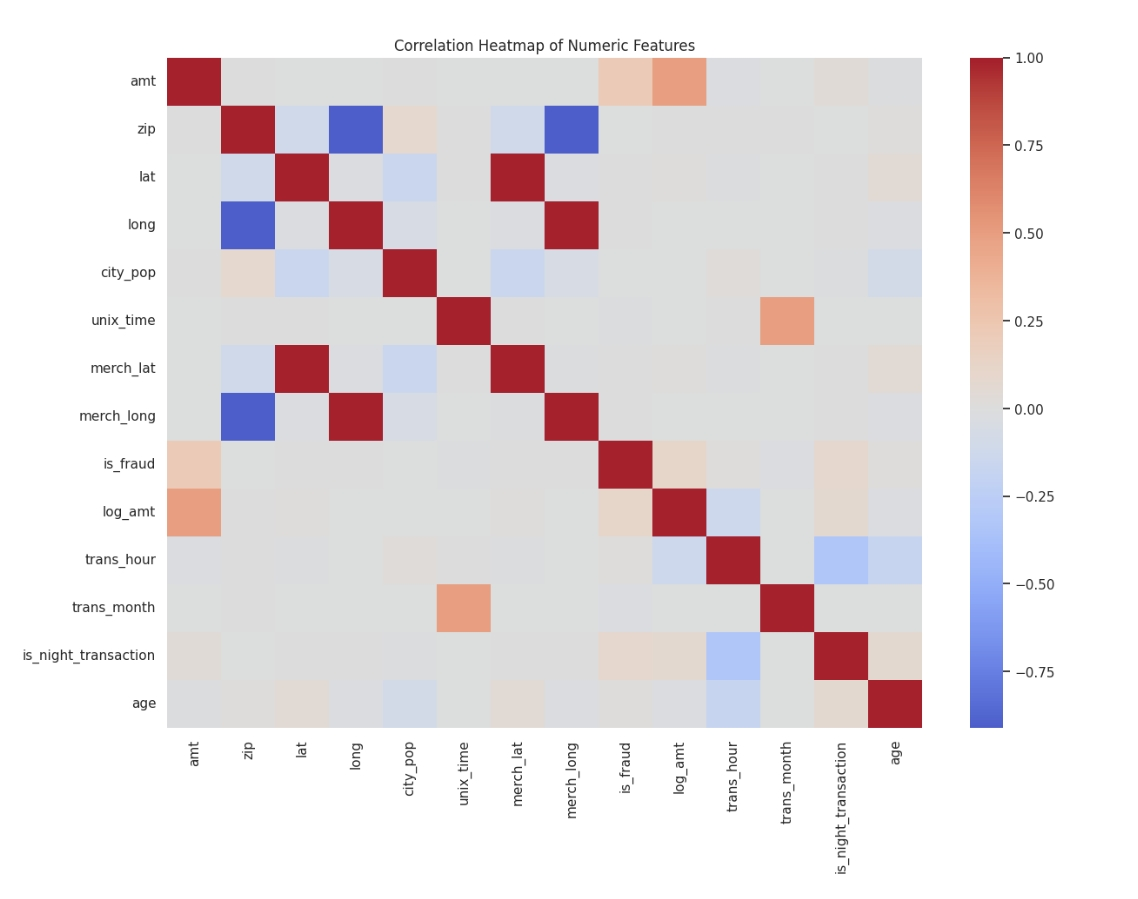
\includegraphics[width=0.8\textwidth]{figures/heatmap.png}
\caption{Correlation Heatmap}
\end{figure}

Most features show weak correlations with fraud, confirming that fraud detection is a multi-feature problem.

\subsection{Top Features Correlated with Fraud}

\begin{figure}[H]
\centering
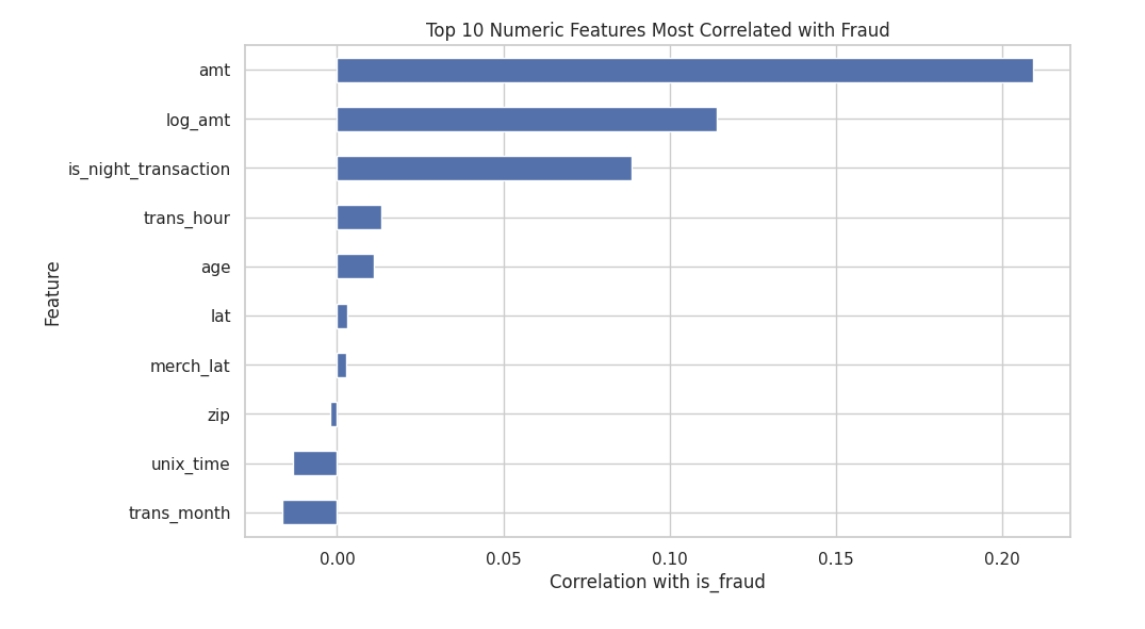
\includegraphics[width=0.8\textwidth]{figures/top_features.png}
\caption{Top Features Correlated with Fraud}
\end{figure}

Transaction amount is the strongest predictor, followed by log-transformed amount and night transaction indicators.

\subsection{Fraud Fingerprint}

A typical fraudulent transaction can be summarized as:

\begin{quote}
A high-value transaction occurring late at night, often in online retail categories, and more likely toward the end of the week.
\end{quote}

\section{Limitations}

\begin{itemize}
    \item Severe class imbalance
    \item Lack of behavioral features (e.g., device, transaction frequency)
    \item Static dataset
    \item Weak linear correlations
\end{itemize}

\section{Implications for Machine Learning}

\begin{itemize}
    \item Use non-linear models (Random Forest, Gradient Boosting)
    \item Engineer temporal and behavioral features
    \item Apply imbalance handling techniques (SMOTE, class weights)
    \item Optimize for precision, recall, and F1-score
\end{itemize}

\section{Conclusion}

Fraud detection is primarily a behavioral problem driven by transaction context rather than demographics. Key indicators include transaction timing, amount, and category.

These insights provide a strong foundation for developing robust fraud detection systems.

\section{References}

\begin{enumerate}
    \item Bolton, R. J., \& Hand, D. J. (2002). Statistical Fraud Detection.
    \item Ngai, E. W. T. et al. (2011). Data mining in financial fraud detection.
    \item Phua, C. et al. (2010). Fraud detection survey.
    \item Chen, C. et al. (2004). Random Forest for imbalanced data.
    \item Kaggle Credit Card Fraud Dataset.
\end{enumerate}

\end{document}

